\documentclass[10pt,letterpaper]{article}

\usepackage{geometry}
\usepackage{hyperref}
\usepackage{graphicx}

\geometry{
  body={7.0in, 10.0in},
  left=0.75in,
  top=0.75in
}

\hypersetup{
  colorlinks = true,
  urlcolor = black,
  pdfauthor = {Alexander Brown},
  pdfkeywords = {},
  pdftitle = {Alexander Brown: CS21120 - Assignment 1: Sudoku},
  pdfsubject = {CS21120 - Assignment 1},
  pdfpagemode = Default
}

\setlength\parindent{0em}
\setlength{\parskip}{1ex plus 0.5ex minus 0.2ex}
\setcounter{tocdepth}{2}

\title{CS21120 - Assignment 1: Sudoku}
\author{Alexander Brown}
\begin{document}
  \maketitle
  \tableofcontents
  \newpage
  \part{Introduction}
    \section{About the Problem}
      The object of this assignment is to produce a peice of software that will solve any possible sudoku in a reasonable amount of time.
      
      The main issue will be balanacing the Completeness of an Algorithm with the Time Complexity (see section~\ref{sec:algorithm_terms} on page~\pageref{sec:algorithm_terms}).
      
      It should be noted that the focus of this assignment is on algorithms, not on the Graphical User Interface (GUI).
      
      \subsubsection{Deadline}
	10am-12noon on the 1st November 2010.
  
  \newpage
  \part{Design}
    \section{Design Choices}
      \subsection{Tile Representation}
	A tile can be represented as:
	
	\subsubsection{Character}
	  Represteting as a character has the advantage of not needing to convert to an interger value. It does have the problem of needing to be converted back to an interger.
	  
	  It also has the advantage of being the input value.
	
	\subsubsection{Interger}
	  Another simple way of representing, 0 would represent the space value in a character.
	  
	\subsubsection{Enumeration}
	  A slightly more complex way would be to use Enumerations, limiting the values which the tile can take.
	
	\subsubsection{Object}
	  Rather than use a predefined type, one could create an Object which held data on a tile. Though this helps encapsulation and is more Object Oriented, it does mean a greater amount of memory needed to represent each sudoku.
	  
	  For some of the more complex algorithms this representation might be prefered as it could hold possible values of the tile, as well as the actual.
	
	\subsubsection{Conclusions}
	  Characters are the most useful of the simple data types. Whilst having an enumeration to limit possible values would be useful to stop bad user input, it is an issue which does not need to be worried about.
	  
	  Intergers have somewhat less use, especially when thinking about converting characters into intergers.
	  
	  Objects may be useful in certain circumstances, but in those circumstances it might be better to create a virtual board and tiles. Esepcially when considering how some of the algorithms using Tree Structures will already use a lot of memory.
	  
	  After Prototyping, it seems simpler just to pick a single type, this will be characters due to their usefulness.
	  
      \subsection{The Representation of the Sudoku Grid}
	There are at least three ways in which to represent the Sudoku Grid:
	\subsubsection{Array}
	  The simplest representation is as a single dimension array. For the vast majority of the algorithms this is possibly the easiest representation, as it allows for simple incramentation, rather than having to play about with 2 or more values.
	
	\subsubsection{Matrix}
	  A more practical approach is to model the sudoku as a 2d array as sudokus themselves are 2d arrays. This allows for ease of getting rows, colomns and, to a certain extent, the \(3\times 3\) sub grids (the latter using interger division). It also has an advantage when displayed graphical of already being in the form it is needed to be in.
	
	\subsubsection{Matricies within a Matrix}
	  The final method would be to represent the \(3\times 3\) sub grids as 2d arrays, then contain them within another 2d array. This only has advantages if the sub grids need a lot of access and should probably only be implemented when using the most complex searching algorithms.
	  
	\subsubsection{Conclusions}
	  Because all representations each have their own uses, it is probably best to create an interface and implement at least the Array and Matrix representations implementing the interface. However if this proves too clumbersome, the Matrix representation is the best middle ground.
	  
	  However after some prototyping, it seems it will be simpler just to chose the Matrix representation.
	  
      \subsection{Graphical Interface}
	Whilst the Command Line Interface can be driven using command line parameters or simple i/o. The Graphical Interface will have to be more complex.
	
	The user will most likely want to see the algorithm act on the grid step by step, run it all the way through or even pause it half way through. They might also want to load in a different sudoku without reloading the program.
	
	Should there be time, these are important issues to deal with and the design should allow for such features.
  
    \section{Unified Modeling Language (UML) Design}
      \subsection{UML Class Diagram}
	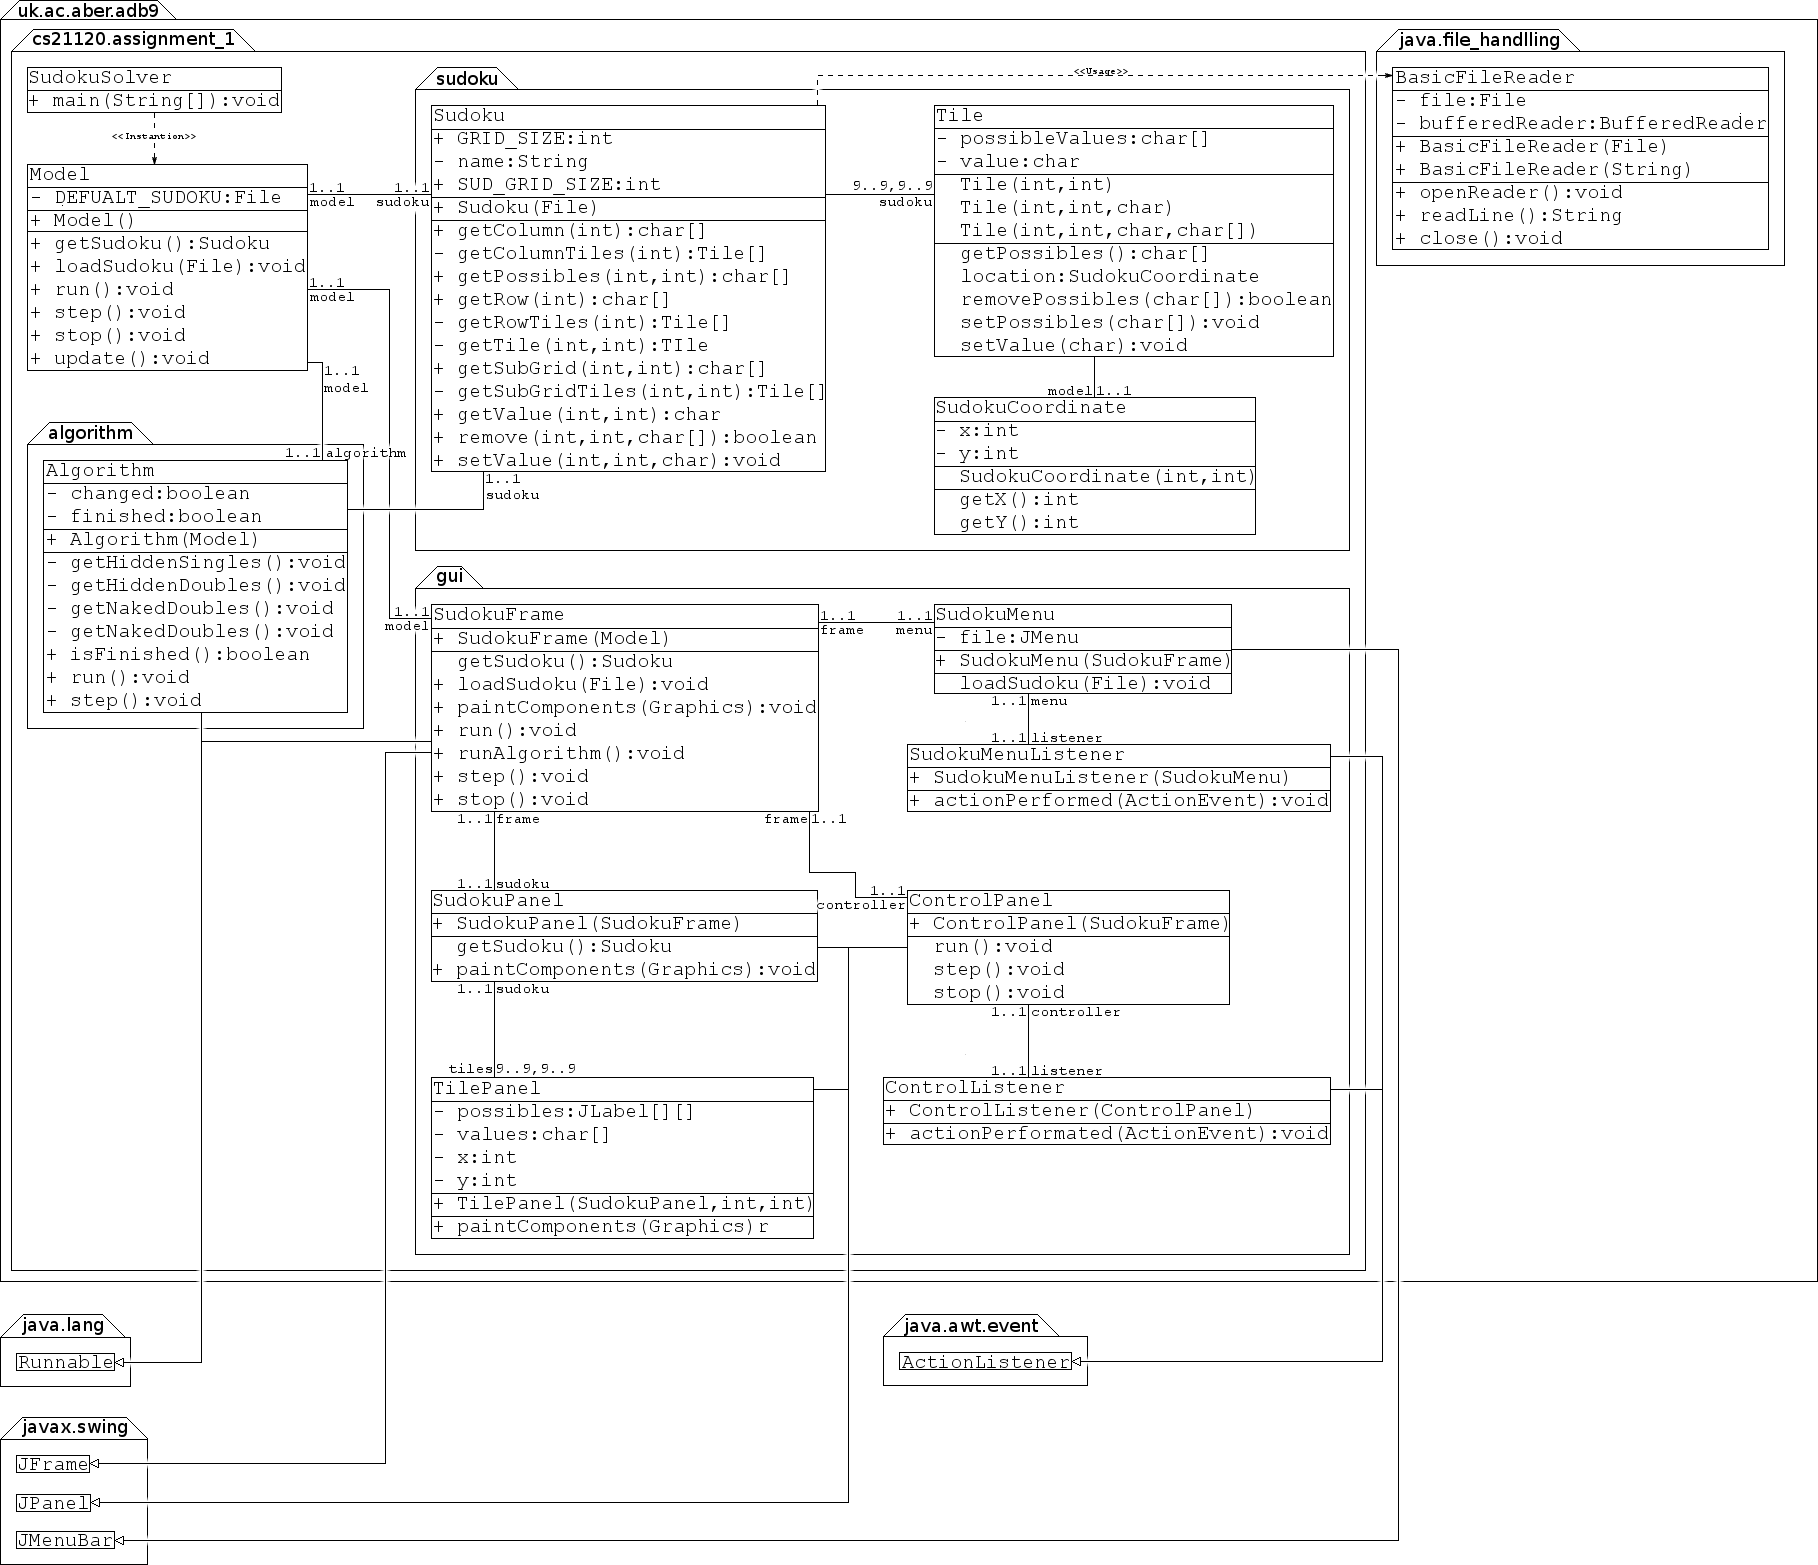
\includegraphics[scale=0.25]{uml.png}
  
  \newpage
  \part{Algorithm Design}
    \section{Overview}
      As a sudoku can be solved without guessing there should be no need for a brute force algorithm. Instead there are several approaches to solving a Sudoku.
    
    \section{Basic Approaches}
      \subsection{Naked Singles}
	Naked singles are the simplest for a computer to find. If, after cancelling possible values by using values in the row, column and sub-grid, a tile has only a single possible value, then that tile must take this possible value.
	
	\subsubsection{Psuedocode}
	  \begin{verbatim}
function nakedSingles()
  for(all tiles)
    get the values of the tiles in this row.
    get the values of the tiles in this column
    get the values of the tiles in this sub-grid
    
    remove all of the above from the possible values of this tile
    
    if(only one possible)
      set the value of the tile to that possible value
	  \end{verbatim}
      
      \subsection{Hidden Singles}
	Hidden singles are possible values in tiles which might have possible values, but which cannot go anywhere else in the row, column or sub-grid that tile is in.
	
	\subsubsection{Psuedocode}
	  \begin{verbatim}
function hiddenSingles()
  for(all tiles)
    get tiles for this row
    getHiddenSingles(tile, row)
    
    get tiles for this column
    getHiddenSingles(tile, column)
    
    get tiles for this sub-grid
    getHiddenSingles(tile, sub-grid)    

function getHiddenSingles(Tile tile, Tile[] tiles)
  for(all possibles in tile)
    if(possible is the only possible of this value in tiles)
      set the value of tile to be this possible
	  \end{verbatim}
	
    \section{More Approaches}
      \subsection{Naked Doubles}
	Doubles are a set of two tiles which can only take the same two possible values in a row, column or sub-grid. These two values then cannot be anywhere else in that row, column or sub-grid, so can be removed and led to naked or hidden singles being found.
      
	\subsubsection{Psuedocode}
	  \begin{verbatim}
function nakedDoubles()
  for(all tiles)
    nakedDoublesInRow(tile)
    nakedDoublesInColumn(tile)
    nakedDoublesInSubGrid(tile)

function nakedDoublesInRow(Tile tile)
  if(tile has 2 possibles)
    get row of this tile
    for(tiles in row (not tile))
      if(row tile has the same two possibles)
	remove(row, tile, row tile, value1, value2)

function nakedDoublesInColumn(Tile tile)
  //As nakedDoublesInRow

function nakedDoublesInSubGrid(Tile tile)
  //As nakedDoublesInRow	

function remove(Tile[] from, Tile not1, Tile not2, char value1, char value2)
  for(all in from)
    if(tile != not1 && tile != not2)
      remove value1 from tile
      remove value2 from tile
	  \end{verbatim}
	  
      \subsection{Triplets, Quads and above}
	Triplets and Quads are based on the same theory as Doubles, they contain a set of numbers which can only go in three or four tiles in a certain row, column or sub-grid, which can then be used to cancel out all other possibles of the same value in the rest of the row, column or sub-grid.
	
	It should be noted that quintets, sextents and so on are possible, but somewhat unlikely due to the small size of the grid.
      
	\subsubsection{Psuedocode}
	  \begin{verbatim}
function nakedTriplets()
  for(all tiles)
    nakedTripletsInRow(tile)
    etc.

function nakedTipletsInRow(Tile tile)
  if(tile has 2 possibles)
    get row of this tile
    for(all tiles in row (not tile))
      if(other value already found)
        if(row tile has one of the two values and a single other value)
          other value = the single other value
      else
        if(row tile has the second of the two values and other value)
          remove(row, tile, row tile1, row tile2, value1, value2, value3)
	  \end{verbatim}
      
      \subsection{Hidden Doubles, Triplets and Quads}
	Working on the same principal as hidden singles, one can use the theory of doubles and above to cancel out other values in a tile with the remainder of the double (or above) in it.
	
	\subsubsection{Psuedocode}
	  \begin{verbatim}
function hiddenDoubles()
  for(all tiles)
    hiddenDoublesInRow(tile)
    etc.

function hiddenDoublesInRow(Tile tile)
  if(tile has 2 possibles)
    get row of this tile)
    
    count = 0
    for(all tiles in row (not tile))
      if(tile contains values)
        count++
    
    if(count == 1)
      other tile.setPossibles(value1, value2)
	  \end{verbatim}
      
      
      \subsection{}
\end{document}